\documentclass[a4paper,11pt]{article}

\setlength{\parindent}{0mm}
\setlength{\oddsidemargin}{-5mm}
\setlength{\evensidemargin}{-5mm}
\setlength{\textwidth}{165mm}
\setlength{\textheight}{230mm}
\setlength{\topmargin}{-10mm}
\setlength{\marginparwidth}{15mm}
\setlength{\marginparsep}{7mm}
\usepackage{float}

%Include some packages which give certain fonts, graphics capabilities, etc
\usepackage{graphicx}% Include figure files
\usepackage{dcolumn}% Align table columns on decimal point
\usepackage{color}% bold math
\usepackage{bm}% bold math
\usepackage[caption=false]{subfig}
\usepackage{listings}
\bibliographystyle{abbrvnat}



\begin{document}



% remove the following for publication
\begin{figure}
\leftline{\hfill }
\end{figure}




% Front matter 
\title{An Experiment Looking at the Temperature Dependence of Second Sound in Helium-II Superfluid}
\author{Samuel Hedges}
\date{09/11/2022}
 \maketitle
 \newpage
\begin{abstract}
In this experiment the temperature dependence of the velocity of second sound of helium was being measured. this involved cooling liquid helium to cryogenic temperature till it underwent a phase change to a bose-einstein condensate at which point heat would travel as entropy waves between the Helium-I (normal fluid) and Helium-II superfluid. In this experiment it was concluded that the velocity of second sound is at a maximum when the temperature is (\appox 1.7K) and thus this is the point when there are equal amounts of Helium-I and Helium-II
\end{abstract}
 \newpage
 \tableofcontents
\newpage

\section{Introduction}
\textbf{The introduction should motivate the work that is described, set it in a wider context and explain why it is important or interesting. The introduction should inspire the reader to read on. The main result may be mentioned as part of this process, but repeating the results of the investigation is not the main function of the introduction.}
\\

\text{Second sound is a quantum mechanical effect where the transfer of heat occurs via a wave like motion rather than the normal diffusion. It can be observed in many different materials but most noticeable for the purposes of this experiment is observations of second sound in Helium-II superfluid. The term "Second Sound" is in reference to the wave like motion of the temperature and Entropy within the Superfluid \cite{Second Sound: The role of elastic waves}.}
\\

\text{Second sound has been found to have uses throughout physics. Oscillating super leak transistors are used throughout industries in the detection of any possible quenching in superconducting wires and magnets. The detection of second sound here can be used to find any defects or cavities that may be present in such materials allowing for reduction of risk and maintenance of such equipment \cite{Tesla Paper}. Another use of second sound is as a thermometer between the temperatures of 0.7K to 0.01K. The second sound harmonic frequency can be recorded as the temperature lowers. Knowing how the frequency changes allows for the use of this as a thermometer at these low temperatures. This application is used at lower temperatures when traditional thermometry is ineffective; This also allows for the prediction of temperature when increasing temperature within the cryostat which isn't able to be done by use of Ideal Gas Laws. \cite{Helium Second Sound Velocity}.}
\\

\text{In the experiment the temperature dependant velocity of the second sound was being measured. The relation between second sound velocity and temperature was found; as the temperature increased the velocity decreased. From research this is the relation that would be expected from research into the prior experiments and by the theory \cite{Liquid Helium}. }

\section{Background: What is Second Sound, and How Does it Come About in Liquid Helium?}

\text{In this experiment Second Sound was being observed in superfluid Helium 4 (which has been and will subsequently be referred to as Helium-II). Superfluid Helium-II only occurs at cryogenic temperatures ($\approx 2.17K$) a cryostat was therefore used to maintain the required temperatures.}
\\

\text{A cryostat is a device that is designed to maintain cryogenic temperatures of samples or devices mounted with it (the cryostat). In this experiment decisions were made relating to the materials used within the cryostat and some of the designs that helped maintain these cryogenic temperatures \cite{Pobell F. Matter and methods at low temperatures}.One of these adaptations was aluminium foil that was wrapped around the outer surface of the cryostat to reflect and inferred radiation incident upon it \cite{Influence of reflectance from flat aluminum}. Another was liquid nitrogen being used to initially cool down the cryostat \cite{A nitrogen cryostat} to cryogenic temperatures before the liquid helium was poured into the cryostat; this allowed for greater control of the boil off rate of the helium and is also safer than pouring liquid helium straight in. A further design element that was taken into account is how the radiation from the cap of the cryostat was controlled, it was calculated that $\approx 1.299 Watts$ would be emitted from the cap. This Radiation was controlled through use of baffles which acted as a thermal barrier absorbing some of this heat as well as controlling the helium gas flow rate so that the majority of this radiation could be absorbed (and thus removed) by the helium gas. Materials used in the cryostat were mainly steel due to its durable properties at lower temperatures. A concerted effort was made so that the metals used had similar thermal expansion; if they are too different this would cause components to crack}
\\

\text{Helium-II is a superfluid state of helium that can be seen when helium is cooled to below 2.17 Kelvin. Superfluidity is a state where there is zero viscosity and thus the fluid can flow without any loss of kinetic energy (due to its own inertia). The phenomena of superfluidity often comes about due to Bose-Einstein condensates (such as superfluid helium 4), but this is not necessary for observations of superfluidity\cite{superfluidity of Bose-Einstein condensates}. A Bose-Einstein Condensate occurs when a gas of bosons inhabits the ground state, under usual circumstances Helium-4 is considered a Fermion but when it drops to its lowest energy state, the electrons and nucleons form spin up and spin down pairs; this gives the atom an overall integer spin therefore it can be treated as boson like with a single wave function describing all the atoms. \\The temperatures at which this state can be observer are shown in Figure \ref{fig:Helium Phase Diagram}.}
\begin{figure}
    \centering
    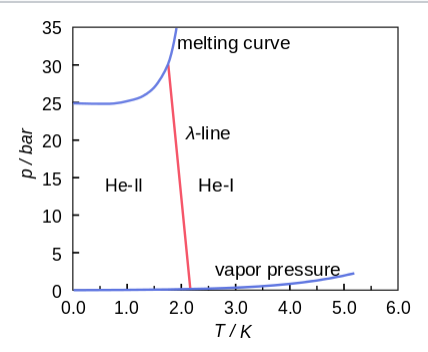
\includegraphics[scale=0.9]{Screenshot 2022-11-29 at 00.03.59.png}
    \caption{This is a figure of a helium phase diagram \cite{Helium Phase Diagram (c)} as can be seen there is a $\lambda$-line that separates out the two different liquid phases of helium. Above this line He-I exists and Helium acts as a normal fluid, below it is He-II }
    \label{fig:Helium Phase Diagram}
\end{figure}
\\

\text{In the He-II phase, below the $\lambda$-line, there is both superfluid helium and normal liquid helium. The behaviour of the two fluid can be described using the two fluids model \cite{Two Fluids Model} with a normal component, and a superfluid component. The ratios of the superfluid component to the normal component will increase as the temperature decreases, and below 1 Kelvin it can be considered to be entirely superfluid helium \cite{Ratio of Superfluid to Normal Helium}. The two components in the Two Fluids model are not able to mix, and will stay separate of one another. When in this state it is possible to create density waves that are of the normal component (and hence the superfluid component because the two components do not mix). This wave acts similar to a normal sound wave and is what is referred to as second sound. It is the velocity of such waves at differing temperatures (and thus different amounts of normal and Superfluid helium) that was being investigated in this experiment.}
\\

\text{In this experiment a germanium thermometer was used. Germanium is a semiconductor and therefore the resistance will increase as the temperature decreases. There are two energy levels in a semiconductor conduction band and valence band. When the semiconductor heats up the electrons in the valence band can break free of their covalent bonds and move to the conduction band as charge carries. As the temperature decreased the electrons lose this energy and drop back into the valence band. The resistance of the germanium was used as a thermometer in this experiment; it was calibrated using the known pressure temperature =relationship when the cryostat is initially pumped.}
\\

\text{The theory of stationary/standing waves was crucial to this experiment. A stationary wave requires two waves travelling in opposite directions with the same (or similar) phase difference and amplitude. the two waves will constructively and destructively interact producing a standing wave which does not travel along the medium. A standing wave has points that do not oscillate called nodes, and points of maximal oscillation called anti-nodes. From first principles using a wave equation, the following equation can be produced for the frequency of the standing wave's oscillation: 
\begin{equation}
        f_n=\frac{n\times v}{2L}
      \label{Standing Wave EQN}  
\end{equation}Where $n$ is the harmonic of the standing wave, $v$ is the velocity, f is the frequency (applied in this experiment), and $L$ is the length of the tube}

\section{Experimental Method: How the Helium was Condensed, and Second Sound Measured}

\text{In this experiment, the following experimental set up was observed.}
\begin{figure}[hbt!]
    \centering
    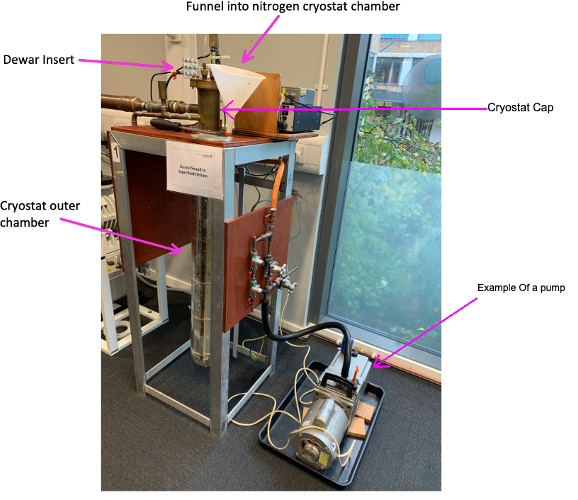
\includegraphics[scale=0.8]{Picture 1.png}
    \caption{A Ladled Picture of the Laboratory's cryostat set-up. In Figure 2, There is: the Dewar insert where the Liquid Helium was pumped in, a cryostat chamber where the liquid helium and liquid nitrogen sit the two thermally insulated from one another, The Liquid Nitrogen funnel where the Liquid nitrogen was pumped in from the liquid nitrogen dewar, The cryostat cap which was removed from the cryostat to measure some of the instruments that were bing used in this experiment, and the Example pump. The one used in the actual experiment is not pictured here, but this is an example of how it would be used to pump out a cryostat; the valves are used to control the pump rate so that too much strain is not put on the pump and so that the cryostat is pumped out safely.}
    \label{fig:Lable Cryostat Picture}
\end{figure}
 \\
\text{To begin, the cap of the cryostat was removed in order to measure the length of the resonance tube where the measurements of second sound velocity took place.}
\begin{figure}[hbt!]
    \centering
    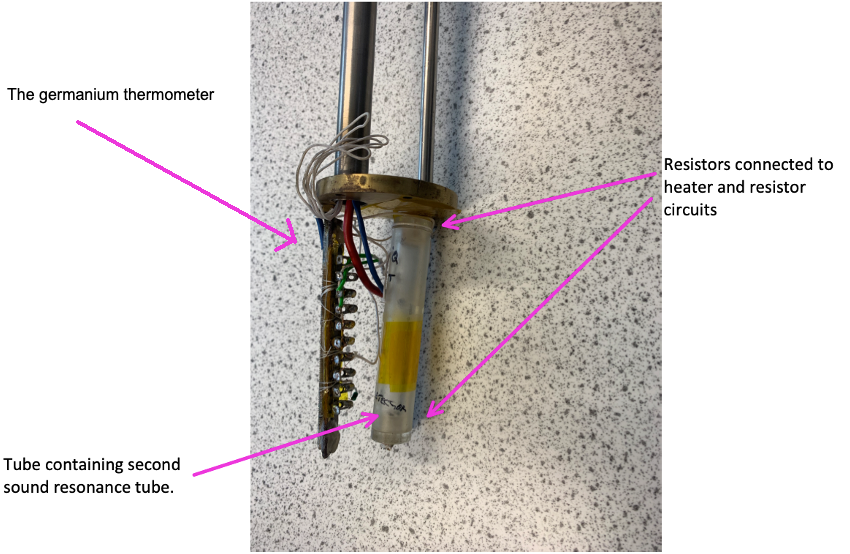
\includegraphics[scale=0.3]{Picture 2.png}
    \caption{Displayed is the insert that was used in the cryostat. Labelled is the germanium thermometer used as the temperature could not be calculated off of thermodynamic variables when it was being increased. The resistors in either end of the tube were used to heat up the tube and thus create the second sound wave that was being measured. This experiment took place in a tube of known size so that the velocity could be found using the standing wave formula (using equation \ref{Standing Wave EQN})}
    \label{fig: Cryostat Insert}
\end{figure}
   \\
   
   \text{The cap was replaced and screwed on. liquid nitrogen was pumped into the outer chamber of the cryostat. This was then left for 45 minutes to cool down the cryostat. This is a necessary step as it cooled down the cryostat meaning that the liquid helium didn't boil off immediately which made the subsequent liquid helium transfer safer and more efficient. the set }
   
   \begin{figure}[hbt!]
       \centering
       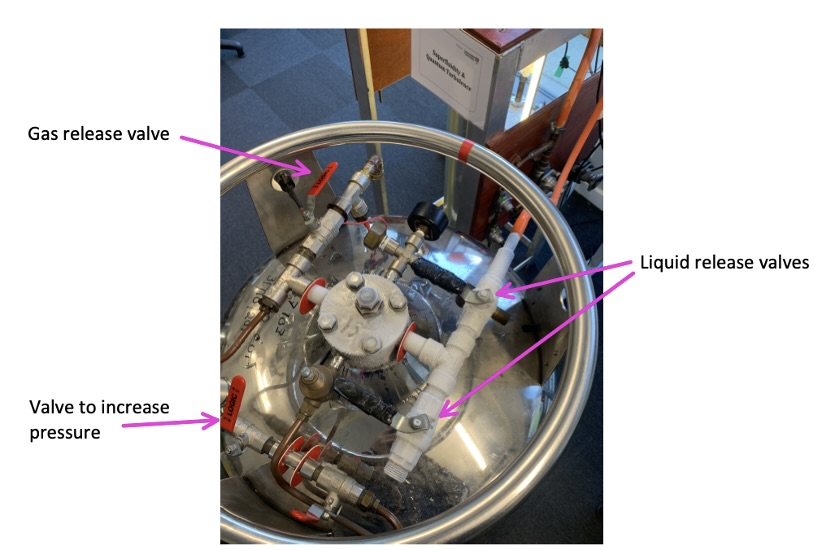
\includegraphics[scale=0.7]{Picture 3.jpeg}
       \caption{Top down image of the dewar. The gas release valve functioned to allow the boil of nitrogen to escape the dewar, ensuring the pressure did not build. When the transfer was taking place, a high pressure was needed inside the dewar to force liquid through the transfer tube, so this was closed pre-transfer. The increase pressure valve released some liquid nitrogen into a copper coil built into the dewar. this allowed nitrogen to boil off at a high rate, which increased the pressure faster which forced more liquid into the transfer tube and thus into the dewar. This increase pressure valve was opened roughly 25$\%$. When the cryostat was filled we first closed the increase flow rate valve, then the liquid transfer tube vale, and finally opened the gas release valve. The set-up for this transfer can be seen pictured in Figure \ref{fig:Liquid Nitrogen set-up}}
       \label{fig:Liquid Nitrogen set-up}
   \end{figure}
   \\
   
   \text{The helium was subsequently pumped into the cryostat. Unlike the liquid nitrogen an insert was used to pump in the helium due to the temperature of the helium. The helium transfer set up can be seen pictured in figure \ref{fig:Helium Transfer} }
   \begin{figure}[hbt!]
       \centering
       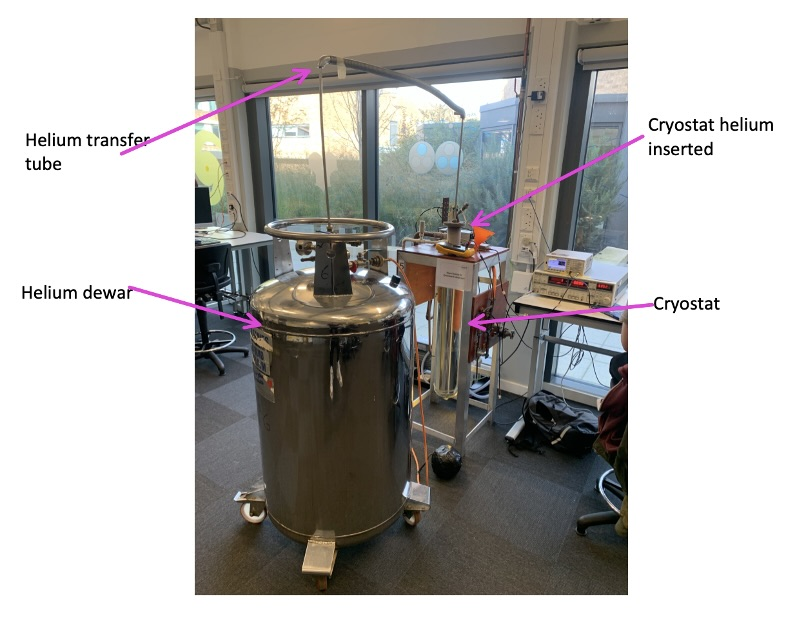
\includegraphics[scale=0.7]{Picture 4.jpeg}
       \caption{Pictured is the helium dewar and the cryostat used. The transfer tube was inserted into the dewar slowly to allow it to cool down.}
       \label{fig:Helium Transfer}
   \end{figure}
   \\
   
   \text{Helium was then pumped into the cryostat attention being paid to the flow rate using the wall mounted monitor. Helium gas was allowed into the cryostat first to cool down the chamber followed by liquid helium till the cryostat had been filled sufficiently. proceeding this the pump was activated. Prior experiments done within the cryostats meant that the temperature of the liquid helium was known as a function of pressure (only when the pressure was being reduced for the first time).The valves to the pump were then open slowly, it was done in this manner so that the pump was not overloaded and so that the germanium thermometer could be calibrated at the known temperatures of the hydrogen. Once the Temperature had dropped to approximately 2.2K a calibration curve was produced. The Resonant frequencies of the first 5 harmonics of the standing wave of second sound was found at 2.2k. This was done by wiring a frequency generator through two resistors either end of the plastic tube that was being used to produce a second sound wave at a given frequency. The resulting oscillations were measured through finding the significantly higher maxima of the standing waves (and using Equation \ref{Standing Wave EQN} once the first was found to get a rough estimate for the others).}
   \\
   
   \text{Next the temperature was increased. This was allowed to happen by tuning off the pump and closing the valves. With the cryostat heating up the standing wave was maintained through slight changes in the input frequency of the resistors. Temperature, and the input frequency of the Second sound wave were measured until the $\lambda$-point was reached. The frequency velocity relation was used to then find the resulting Velocity/Temperature graph for the second sound in Helium-II}
   
\section{Results and analysis: Did the measurements of Second Sound match the model?} 
\text{When the temperature was being reduced initially a calibration curve was produced for the germanium thermometer. From theory, we expect this curve to be logarithmic in nature due to the switching of electrons between the valance and conduction bands of the semiconductor. The graph Figure \ref{fig: Callibration Curve} was produced}

\begin{figure}[hbt!]
    \centering
    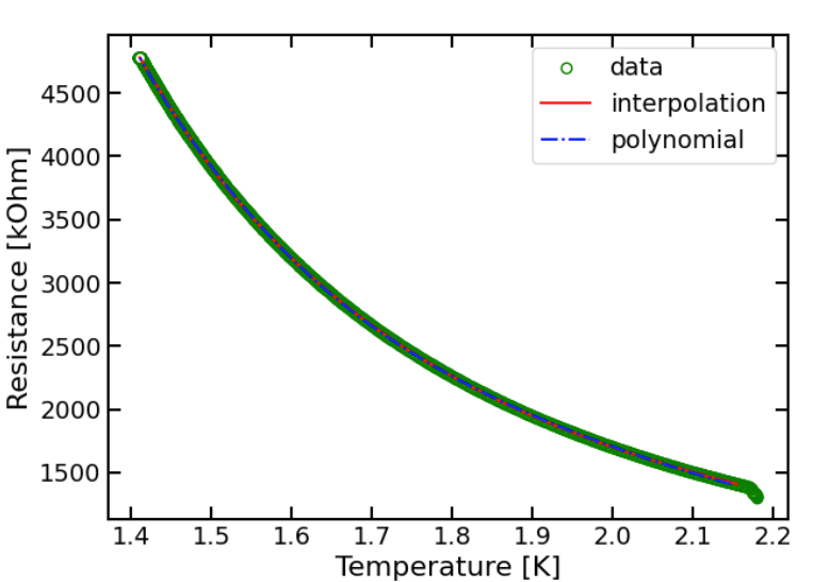
\includegraphics[scale=0.8]{Picture 5.png}
    \caption{A graph of the calibration curve for the Germanium thermometer}
    \label{fig: Callibration Curve}
\end{figure}
\\

\text{The shape of this curve shows that it partially agrees with the experiment. From theory a logarithmic curve was expected and that is what was produced by the data. This agreement means that the thermometry used in this experiment can be said to be repeatable and reproducible. From research into other experiments using germanium thermometers, this calibration curve can be said to have matched roughly what has been produced; this gives further credence to the reproducibility of this part of the experiment \cite{Germanium thermometer}.}

\text{When the cryostat had been pumped out fully, measurements of second sound were taken. These measurements were of the first 5 harmonics.}
\begin{table}[hbt!]
    \centering
    \begin{tabular}{|c|c|c|}
         \hline
         harmonic & Frequency $Hz$ & Uncertainty in Frequency $Hz$ \\
         \hline
         1 & 77.34 & 0.01 \\
         2 & 145.93 & 0.03\\
         3 & 216.55 & 0.03\\
         4 & 287.3 & 0.1\\
         5 & 358.6 & 0.1 \\
         \hline
    \end{tabular}
    \caption{A table of the harmonic frequencies of the helium second sound taken at 1.5 Kelvin (the lowest point the cryostat reached in this experiment). This was plotted to produce figure \ref{fig: 5_Harmonics_Plot}}
    \label{tab: 5_Harmonics_table}
\end{table}
\begin{figure}[hbt!]
    \centering
    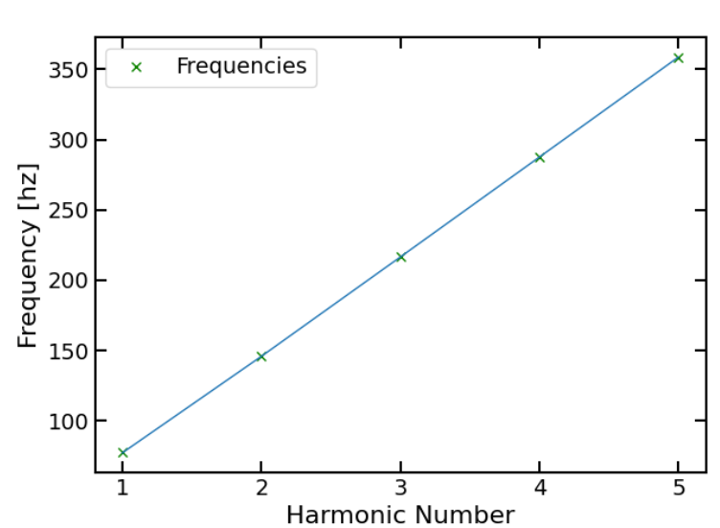
\includegraphics[scale=0.8]{Picture 6.png}
    \caption{A plot of the different harmonics of helium second sound at 1.5K. This plot has a linear gradient and a y-intercept of 5.98+/-0.01 Hz}
    \label{fig: 5_Harmonics_Plot}
\end{figure}
\text{From this graph we can conclude that this experiment partially agrees with the given model of second sound. The linear fit (constant gradient) is what would be expected. Looking at Equation \ref{Standing Wave EQN} it can be rearranged to find the gradient to be: $\frac{v}{2L}$, at constant temperature both $v$ and $L$ will be constant which shows that this experiment agrees with the theory and thus can be said to be accurate and reproducible.\\
Despite this agreement, the non-zero y-intercept disagrees with the theory. The model would expect the frequency to be zero at the "zeroth harmonic". One reason for this non-zero harmonic may be the fact that the entirety of the tube was not being used. This can be due to a build up of Helium-I at one end of the tube so that the second sound wave is not able to oscillate throughout the entirety of the tube, another reason being that impurities can build up in the tube which can also act to shorten the effective length of the tube.\\
This systematic error can now be subtracted from any further measurements made in the cryostat}
\\

\text{The final part of this experiment involved increasing the temperature, and measuring the change in the velocity of the second sound. Figure \ref{fig: Vel_Sans_Sys} was produced from completing the Experimental method previously outlines.}
\begin{figure}[hbt!]
    \centering
    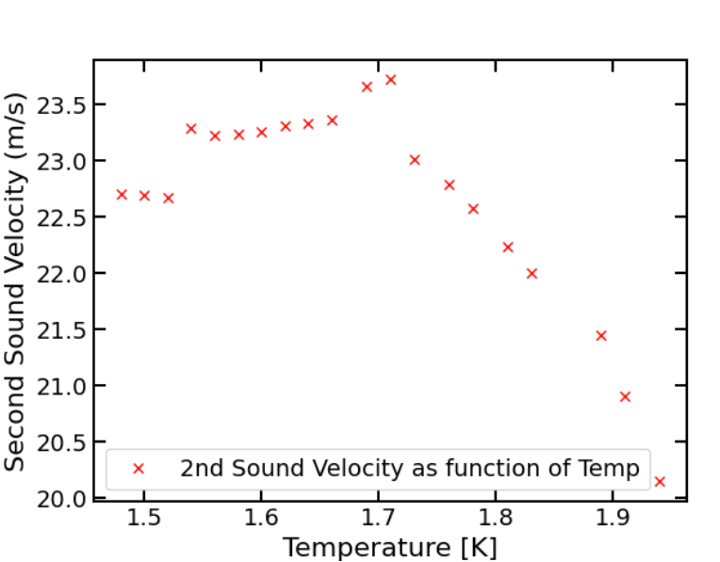
\includegraphics[scale=0.5]{Picture 7.png}
    \caption{A table showing the dependence of the second sound wave's velocity on temperature}
    \label{fig: Vel_Sans_Sys}
\end{figure}
\text{With the knowledge of the systematic error this was subtracted from this graph to produce the final graph that accounted for this systematic error. The systematic error was converted to frequency using Equation \ref{Standing Wave EQN}}
\begin{figure}[hbt!]
    \centering
    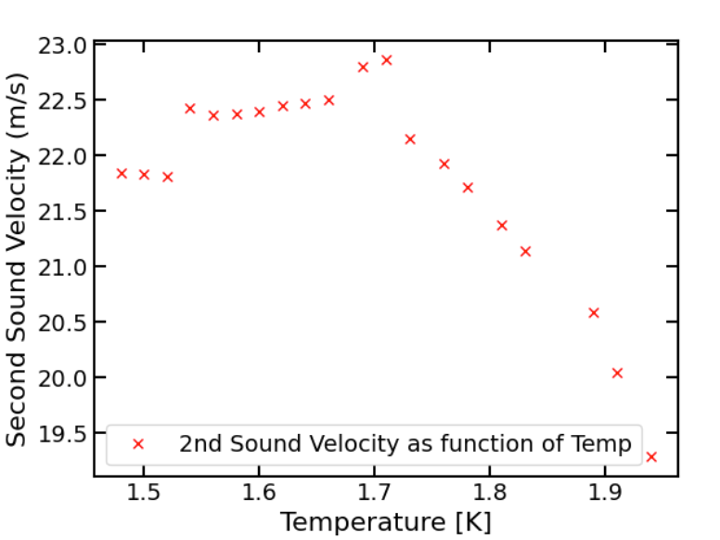
\includegraphics[scale=0.6]{Picture 8.png}
    \caption{A table showing the dependence of the second sound wave's velocity on temperature but has been corrected for the previously found systematic error by subtracting 5.98$Hz$ from all the data points. The peak of the distribution is $22.9\pm0.6ms^{-1}$ and occurs at $\approx1.7K$}
    \label{fig: Vel}
\end{figure}
\text{Looking at figure \ref{fig: Vel}, we see the expected curve. The velocity initially increased to a maximum (peak) at $\approx1.7K$ then decreases to zero at $\approx 2.1K$. Both of these behaviours are explainable using the second sound model. The maximum occurs when there is near equal amount of Helium-I and Helium-II for the Second sound to propagate through, where there are higher amounts of either the second sound is going to be slower due to the lack of the other (i.e. When there is more Helium-II there is less Helium-II to propagate through). THe decreasing to a minimum occurs due to the $\lambda$-transition point, after this point there is only Helium-I and therefore a second sound wave can no longer be sustained.\\
The value for the peak was given as $22.9\pm0.6ms^{-1}$ Using Data obtained from other groups who did this experiment as well as other pieces of work \cite{Lab-book} the true value for this peak was given as $20.4ms^{-1}$.\\

The experiment does not agree with this within one standard error we therefore cannot say that the experiment has agreed with the figure obtained and thus cannot be said to be reproducible. Some reason for this disagreement may be that the systematic error that was obtained from taking the harmonics could be different at different amounts of Helium-II and thus has greater effect at the peak of the velocity (when there is the most Helium-II). This disagreement may also come from the measurement itself, it was done by manually altering the frequency to stay on the peak, this was very empirical and allowed for disagreement within the group of where the actual peak was; as a result this may have effected the readings taken. In future experiments an improvement can be made through either a better way of determining the peak or by using greater uncertainties to match the internal disagreement.}
\\

\text{Some further improvements that can be made to this experiment are as follows. The first improvement is that the measurements that produced the curve seen in Figure \ref{fig: Vel} could be repeated. This does come with a time commitment, but would allow for more group members to take the peak as well as allowing for the removal of any anomalous results. A further improvement would have been to continue until the actual $\lambda$-point was reached, this would have allowed for another figure to measure the reproducibility of this experiment against and further test the theory}

\section{Conclusion}
\text{To conclude, in this experiment the velocity of second sound as a function of temperature was being researched. This was done by increasing the temperature of the experiment form $\approx 1.5K$ to $\approx 2.1K$ and measuring how the harmonic frequency of the temperature would change. Using the harmonic frequency equation (Equation \ref{Standing Wave EQN}) The velocity of the second sound harmonic wave was calculated allowing for the production of a curve (\ref{fig: Vel}). From this curve we can see that the second sound has a polynomial property, where it increases to a maximum and then decreases to 0Hz due to the lack of either Helium-I, or Helium-II due to too low or high temperature respectively. The peak of this graph represents the point at which there are near equal amounts of Helium-I and Helium-II. This peak was calculated to be $22.9\pm0.6ms^{-1}$. This did not agree with the other experiments or the  within one standard uncertainty and therefore cannot say that this experiment is reproducible. Some improvements that could be made that would have made it more likely to be reproducible would be to taken repeat measurements and to take measurements over a longer temperature scale which would allow for the elimination of outliers and to find the point at which the amount of helium-II superfluid dropped to zero which could be compared between experiments}

\newpage
\section{Bibliography}
\begin{thebibliography}{99}
    
    \bibitem{Second Sound: The role of elastic waves} Srinivasan R. Second sound. Resonance. 1999 Jun;4(6):15-9.
  
    \bibitem{Tesla Paper} Conway ZA, Hartill DL, Padamsee HS, Smith EN. Oscillating superleak transducers for quench detection in superconducting ILC cavities cooled with He-II. Proceedings of LINAC08, Victoria, BC, Canada THP036. 2008 Sep.
   
    \bibitem{Helium Second Sound Velocity} Maurer RD, Herlin MA. Second sound velocity in helium II. Physical Review. 1949 Oct 1;76(7):948.
    
    \bibitem{Pobell F. Matter and methods at low temperatures}Pobell F. Matter and methods at low temperatures. Springer Science \& Business Media; 2007 Feb 15.
   
    \bibitem{Liquid Helium}Wilks J. The Properties of Liquid Helium.
   
    \bibitem{Influence of reflectance from flat aluminum}Kostic LT, Pavlovic TM, Pavlovic ZT. Influence of reflectance from flat aluminum concentrators on energy efficiency of PV/Thermal collector. Applied Energy. 2010 Feb 1;87(2):410-6.
   
    \bibitem{A nitrogen cryostat}Meletov KP. A nitrogen cryostat with adjustable temperature and cold loading of samples for the measurement of optical spectra. Instruments and Experimental Techniques. 2020 Apr;63(2):291-3.
    
    \bibitem{Encyclopedia of condensed matter physics. Amsterdam: Elsevier; 2005}Bassani GF, Liedl GL, Wyder P, editors. Encyclopedia of condensed matter physics. Amsterdam: Elsevier; 2005.
    
    \bibitem{Helium Phase Diagram (c)}1. Inkscape O authored by w:en:User:AdwaeleConverted to svg by w:ja:User:KtnsiThe source code of this S is valid T vector image was created with. English:  Phase diagram of helium four$日本語$: $ヘリウム4の相図$ [Internet]. Wikimedia Commons. 2012 [cited 2022 Nov 28]. Available from: https://commons.wikimedia.org/w/index.php?curid=41785150
    
    \bibitem{Two Fluids Model}Feynman RP. Atomic theory of the two-fluid model of liquid helium. Physical Review. 1954 Apr 15;94(2):262.
  
    \bibitem{Ratio of Superfluid to Normal Helium}Landau L. Theory of the superfluidity of helium II. Physical Review. 1941 Aug 15;60(4):356.
  
    \bibitem{superfluidity of Bose-Einstein condensates} Singh VP, Weimer W, Morgener K, Siegl J, Hueck K, Luick N, Moritz H, Mathey L. Probing superfluidity of Bose-Einstein condensates via laser stirring. Physical Review A. 2016 Feb 22;93(2):023634.
    
    \bibitem{Germanium thermometer} Willey DR, Crownover RL, Bittner DN, De Lucia FC. Very low temperature spectroscopy: The pressure broadening coefficients for CO–He between 4.3 and 1.7 K. The Journal of chemical physics. 1988 Aug 15;89(4):1923-8.
    
    \bibitem{Lab-book}Enss, C., and S. Hunklinger. 2005. Low-Temperature Physics. Springer Verlag.
McClintock, P. V. E., D. J. Meredith, and J. K. Wigmore. 1984. Matter at Low Temperatures. Blackie.
\end{thebibliography}
\end{document}